\documentclass{llncs}
\usepackage{graphicx}
\newcommand{\lab}[1]{\textsf{#1}}
\newcommand{\blab}[1]{\lab{\bfseries #1}}
\newcommand{\ilab}[1]{\lab{\itshape #1}}
\begin{document}
\title{Experimenting with Reaction Systems using Graph Tansformation}
\author{Roberto Bruni$^1$ \and Arend Rensink$^2$}

\institute{
University of Pisa, Italy,
\email{bruni@di.unipi.it} \and
University of Twente, Netherlands,
\email{arend.rensink@utwente.nl}}
\maketitle

\emph{Roberto: some general text about Reaction Systems, their usefulness but also the difficulties inherent in their analysis}

Graph Transformation is a modelling technique that is widely applicable in problem domains where the objects of study have an inherent graphical structure, meaning that they can be naturally though of as consisting of nodes (of some kind) linked by edges (of some kind), and the task at hand is to study their properties and evolution. Besides the graphs themselves, the core concept is that of a (transformation) \emph{rule} capturing a particular change to such a graph. Rules can be used, for instance, to describe the change of a system over time, but can also be instrumental in composing and decomposing the graphs and in that manner expose structural properties.

Importantly for the utility of the technique, there are a number of (academic) tools supporting their use. The research described here crucially relies on GROOVE, one of the most prominent tools in this area, which was designed precisely to enable Graph Transformation-based system analysis of the kind described above. In particular, a feature of GROOVE that is essential for the purpose of this reseach is the ability to formulate \emph{nested} (or \emph{quantified}) rules, which capture simultaneous changes in all neighbourhoods that satisfy certain application conditions, rather than only local (single) changes in one such neighbourhood at a time. Another feature is the ability to \emph{explore} the set of reachable graphs (under the given rules) using various strategies.

We are in the process of investigating how Graph Transformation can help in addressing the analysis questions in Reaction Systems. For this purpose, we have defined an encoding of a given RS system as a single graph, upon which a small number of (fixed) rules operate to simulate the correct semantics. The core rule describes describes the simultaneous firing of all \blab{Reaction}s, given that none of their \lab{inhibitor}s are present whereas all of their \lab{reactant}s are present; the firing results in the presence of all \lab{product}s. Simultaneously, all currently present \blab{Entity}s are removed. In GROOVE syntax, this looks as follows:

\begin{center}
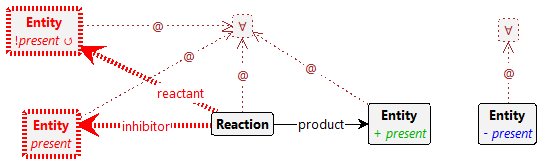
\includegraphics[scale=.6]{react}
\end{center}

To parse this, note that (in the GROOVE rule syntax) the red structure constitutes an application condition requiring its absence; moreover, green labels are added and blue ones deleted upon rule application. The \ilab{present} flag signals whether an \blab{Entity} is considered to be currently present; hence, creating or deleting that flag comes down to creating or deleting the \blab{Entity}. The $\forall$-nodes impose the desired quantification, causing a single application of this rule to model the firing of all enabled \blab{Reaction}s, even if there are thousands of them.

Our model also supports environments that inject \blab{Entity}s in a controlled manner. This is achieved through a second rule, not shown here. A configuration is reachable if it can be constructed by the alternating application of both rules.

\medskip\noindent
Our first results are encouraging: the capability of GROOVE to explore larger Reaction Systems is well beyond what other tools have been able to achieve, meaning that we are often able to find unwanted patterns in reachable configurations (if they exist); moreover, given a trace to such an unwanted pattern, we can also extract the causal history of the entities, at least as far as reactants are concerned.
\end{document}
